% -----------------------------------------------------------------
% => Ambiente Externo
% -----------------------------------------------------------------

\subsection{Ambiente Externo de Aprendizagem}
\label{section:OutdoorClassroom}

\cite{Xue:2011} descrevem um \textit{framework} para criação de ambiente de aprendizado ubíquo baseado em Internet das Coisas e com três camadas: percepção, rede de computadores e aplicação. Apesar de não utilizar um sensor específico, este trabalho indica elementos que podem ser utilizados para construir um ambiente de aprendizado ubíquo e que seja integrado com qualquer sensor ou aplicação (Figura~\ref{fig:Xue2011}).

\begin{figure}[ht]
	\centering
	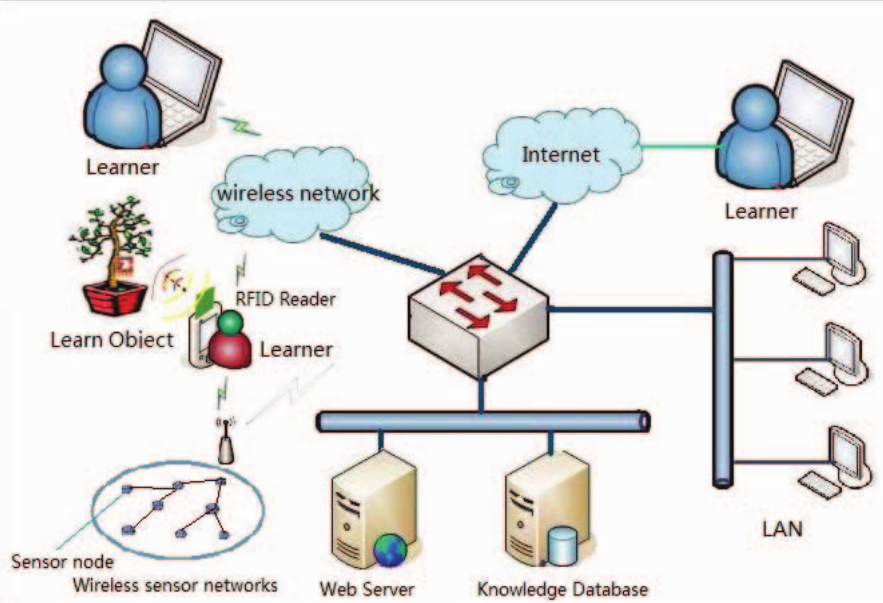
\includegraphics[width=0.9\linewidth]{imgs/Xue2011}
	\caption{Arquitetura do Sistema de Aprendizagem Ubíqua}
	\label{fig:Xue2011}
\end{figure}

\cite{Oluwagbemi:2014} apresentam uma revisão de literatura acerca das tendências da aplicação de métodos de computação pervasiva em ambientes de sala de aula apresenta trabalhos focados em \textit{3D Printing}, \textit{Quantified Self}, Assistentes Virtuais, Jogos e \textit{Gamification}. Como trabalhos futuros é sugerida a adoção e implementação de um modelo nigeriano de ambiente de aprendizado em sala de aula.

\cite{Dong:2007} apresentam um método de reconhecimento de contexto de aprendizagem baseado na Análise do Comportamento para recomendação de um calendário de estudos, quando o estudo é feito em casa, com o objetivo de incentivar o estudante a adquirir o hábito da aprendizagem. O trabalho utiliza sensores de RFID para detectar se os livros estão sobre a mesa de estudo e o sistema cruza essa informação com os dados dos professores e a demanda dos pais para considerar se o aluno está ou não em um contexto de aprendizagem. Se estiver, então, uma programação de estudos é feita pelo sistema. Entretanto, a avaliação do desempenho do sistema foi feita através de formulários aplicados aos estudantes, onde mais de 80\% concordou que o sistema proposto contribui para a melhoria do processo de aprendizado.

\cite{Tan:2007} propõem utilizar a tecnologia em ambientes de aprendizagem externa para ajudar num maior ganho educacional. Utilizando os conceitos de aprendizagem móvel, aprendizagem ubíqua e reconhecimento de contexto foi desenvolvido um sistema denominado "\textit{Ubiquitous Learning with Educational Resources}"~(EULER) baseado em RFID, Internet, redes sem fio, sistemas embarcados e tecnologias de Banco de Dados.

\begin{figure}[ht]
	\centering
	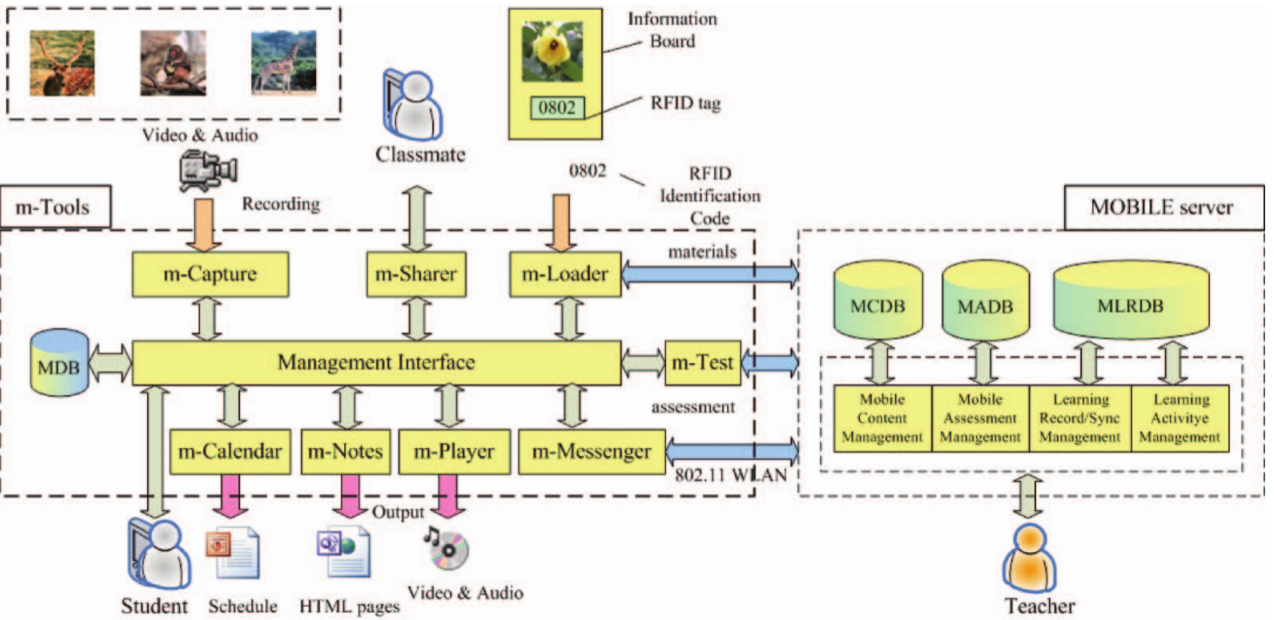
\includegraphics[width=0.8\linewidth]{imgs/Tan2007a}
	\caption{Estrutura do sistema EULER}
	\label{fig:Tan2007a}
\end{figure}

O sistema EULER consiste em dois subsistemas (Figura~\ref{fig:Tan2007a}): (a) Servidor "\textit{MObile-Based Interactive Learning Environment}"(MOBILE) para uso do professor; (b) ferramentas móveis para os estudantes (m-Tools). O professor prepara e armazena o material didático (que pode conter temas, imagens, áudios e descrição textual) no servidor, construindo as relações entre este e os códigos RFID. Os alunos podem coletar e compartilhar dados, além de editar artigos ao seu próprio critério. Dentre as ferramentas do \textit{m-Tools} que os estudantes podem usar estão: PDA, leitor RFID e câmera.

Com tudo configurado, a aula pode acontecer em qualquer ambiente externo, seja um museu, um zoológico ou um parque. A Figura~\ref{fig:Tan2007b} apresenta um cenário de uso do EULER no \textit{Guandu Nature Park} em Taiwan.

\begin{figure}[ht]
	\centering
	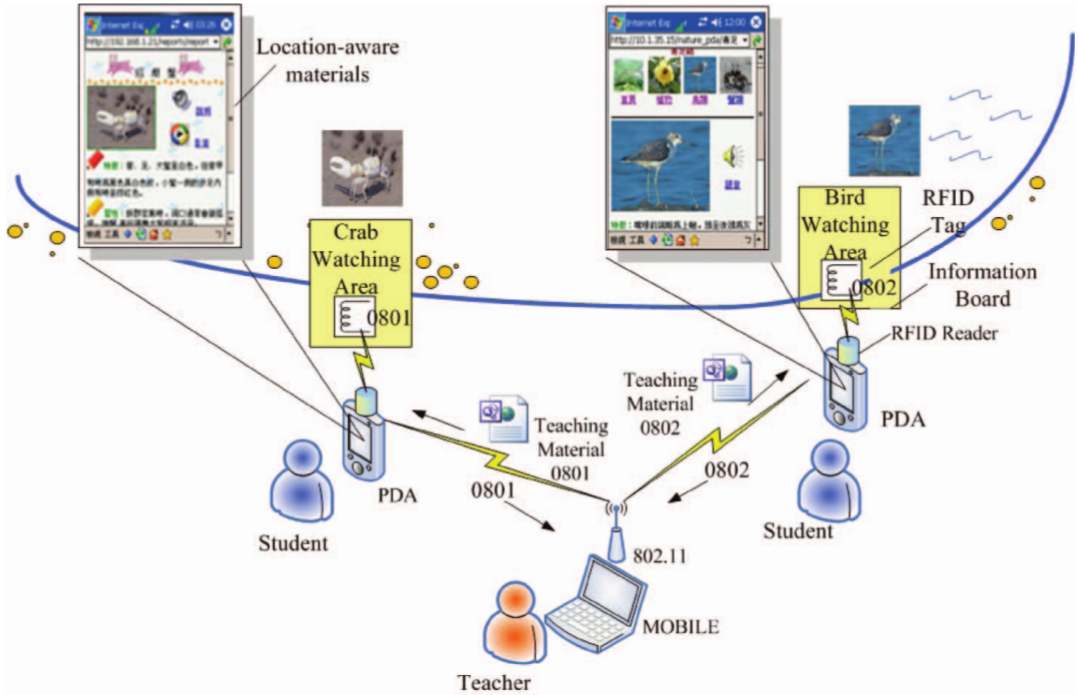
\includegraphics[width=0.9\linewidth]{imgs/Tan2007b}
	\caption{Cenário de uso do sistema EULER no Guandu Nature Park}
	\label{fig:Tan2007b}
\end{figure}

Os experimentos foram executados com dois grupos de 36 alunos cada e o auxílio de quatro professores experientes em educação com uso de computadores. Um grupo experimental utilizou o EULER e um grupo de controle recebeu instrução tradicional. Os experimentos foram divididos em quatro fases e foram aplicados testes antes, durante e depois dos experimentos, com exceção do pré-teste, os estudantes que utilizaram o EULER obtiveram maior desempenho em todos os testes das quatro fases.